\chapter{Tópicos de gerenciamento de requisitos}

\section{Rastreabilidade de requisitos}

	Rastrear requisitos é uma atividade que nos permite controlar e visualizar cada parte do processo e garantir que cada parte do
  desenvolvimento está correto, podemos garantir assim que somente atividades necessárias foram produzidas.

	Rastrear os requisitos através dos estágios de implementação, arquitetura, desing, implementação e teste é importante para garantir a
  qualidade do software. A habilidade de rastrear os relacionamentos e analisar os impactos causados pelas mudanças é crucial
  principalmente para atividades que envolvam sistemas críticos. Requisitos que não estão claros podem causar grandes impactos na
  segurança do projeto e causar um produto não confiável.

  A finalidade de estabelecer rastreabilidade é ajudar a:

  \begin{itemize}
    \item Compreender a origem dos requisitos
    \item Gerenciar o escopo do projeto
    \item Gerenciar mudanças nos requisitos
    \item Avaliar o impacto no projeto da mudança em um requisito
    \item Avaliar o impacto da falha de um teste nos requisitos (isto é, se o teste falhar, talvez o requisito não seja atendido)
    \item Verificar se todos os requisitos do sistema são desempenhados pela implementação
    \item Verificar se o aplicativo faz apenas o que era esperado que ele fizesse.
  \end{itemize}

	A definição sobre rastreabilidade da IEE fala sobre a relação do grau de um elemento com o próximo e como cada elemento tem um objetivo
  bem definido. A rastreabilidade de requisitos pode ser definido então como relação que dois elementos possuem em um mesmo projeto e
  como estes estão conectados.

	Podemos utilizar várias técnicas para rastrear os requisitos, optamos por usar a rastreabilidade horizontal e vertical, entendemos
  que elas são claras e diretas, podemos ter uma visão muito boa a partir dessas técnicas.

	\textbf{Rastreabilidade horizontal} $-$ É a rastreabilidade entre diferentes versões ou variações de requisitos, ou outros artefatos,
  em particular uma fase do ciclo de vida\cite{tese_doutorado}.

	\textbf{Rastreabilidade vertical} $-$ É a rastreabilidade realizada entre requisitos e artefatos produzidos pelo processo de
  desenvolvimento ao longo do ciclo de vida do projeto.\cite{tese_doutorado}.

  \begin{figure}[!h]
    \centering
    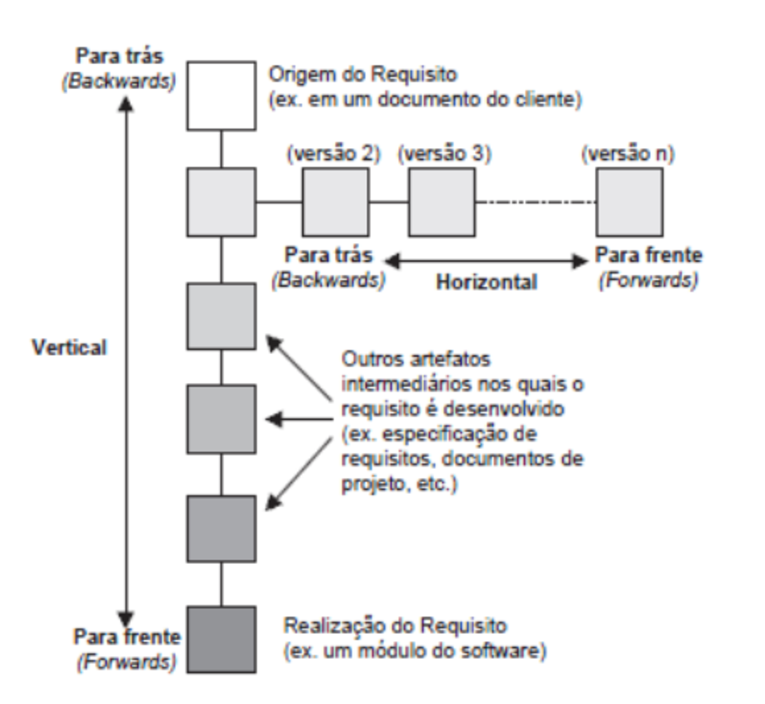
\includegraphics[width=10cm, keepaspectratio=true]{figuras/gerenciamento/rastreabilidade.eps}
    \caption{Rastreabilidade Horizontal e Vertical}
  \end{figure}

  A rastreabilidade horizontal será das versões de cada tema, epico, features e etc, por exemplo, epico 1.1, epico 1.2, e a
  rastrabilidade vertical será a hierarquia mostrada na imagem abaixo, na qual inicial no tema de investimento e termina nas
  tarefas da historia de usuário, tendo assim uma rastreabilidade eficiênte.

  \begin{figure}[!h]
    \centering
    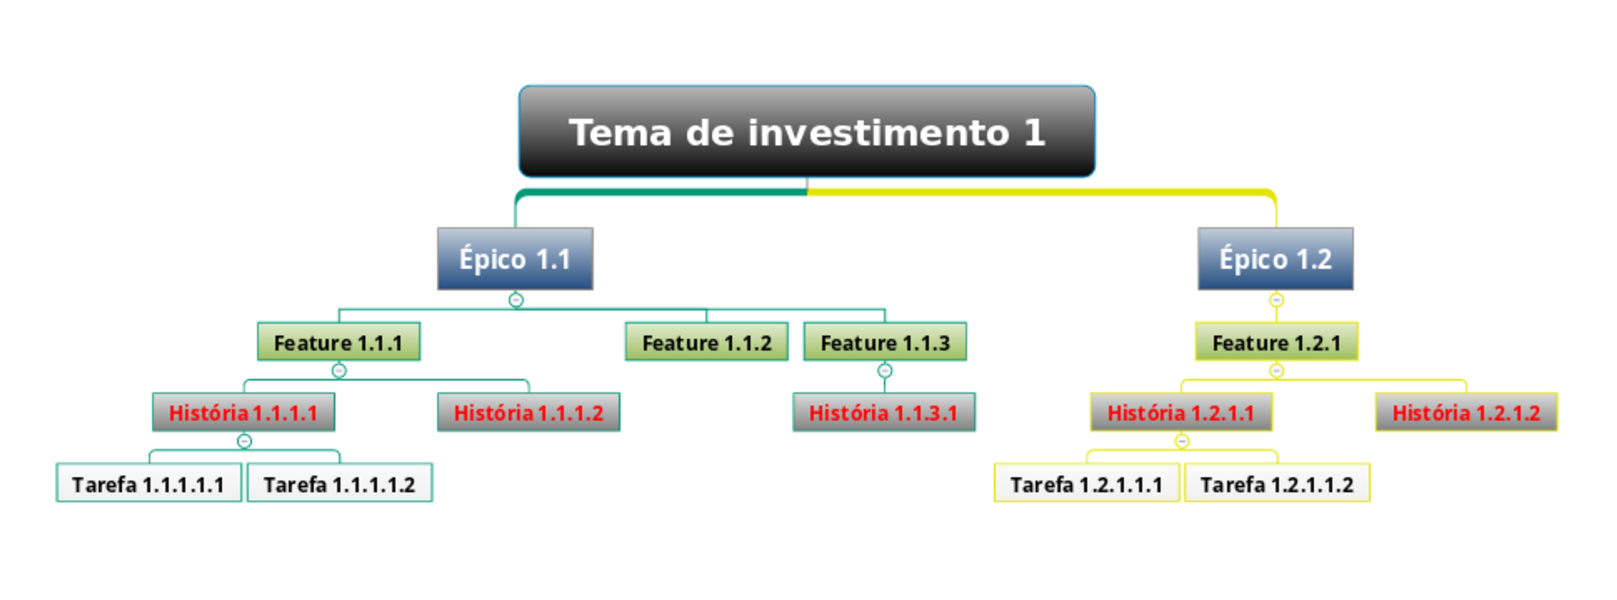
\includegraphics[width=15cm, keepaspectratio=true]{figuras/gerenciamento/temas.eps}
    \caption{Rastreabilidade dos requisitos}
  \end{figure}

\section{Atributos do requisitos}

  Os atributos contém as informações mais importantes daquele requisito, suas propriedades, a partir da qual teremos informações sobre:
  data de criação, origem, entre outras coisas. Os atributos permitem que sejam realizadas consultas dentro de todos os requisitos.

  Os atributos que definimos para gerenciar os requisitos foram:

\subsection{Prioridade}

  Quão importante são os requisitos para os stakeholder e para o sistema

  \begin{table}[!htb]
    \centering
    \begin{tabular}{p{5cm}p{10cm}}
      \toprule
      \textbf{Alta}  & Indica um requisito sem o qual o sistema não entra em funcionamento.                             \\ \midrule
      \textbf{Média} & Indica um requisito sem o qual o sistema entra em funcionamento, mas de forma não satisfatória.  \\ \midrule
      \textbf{Baixa} & Indica um requisito que não compromete as funcionalidades básicas do sistema                     \\
      \bottomrule
    \end{tabular}
    \caption{Atributo de Prioridade}
  \end{table}

\subsection{Estabilidade}

  Este atributo está relacionado com a possibilidade do requisito ser modificado ao longo do projeto e/ou tempo de vida do sistema.

  \begin{table}[!htb]
    \centering
    \begin{tabular}{p{5cm}p{10cm}}
      \toprule
      \textbf{Alta}  & Indica um requisito muito estável, ou seja, é pouco provável que o requisito em questão sofra
                       mudança no decorrer do projeto                                                                       \\ \midrule
      \textbf{Média} & Indica um requisito que tem uma probabilidade 50\% de sofrer alguma mudança                          \\ \midrule
      \textbf{Baixa} & Indica um requisito não estável, ou seja, é muito provável que o requisito em questão necessite
                       de alguma mudança no futuro                                                                          \\
      \bottomrule
    \end{tabular}
    \caption{Atributo de Estabilidade}
  \end{table}

\subsection{Esforço}

	Uma estimativa feita de dificuldade para implementar um requisito. Uma carta com dificuldade proporcional ao requisito implementado,
  Planning Poker, jogo de carta, na qual a equipe irá atribuir um grau de dificuldade para a tarefa de acordo com a sequência de
  fibonacci

  \begin{table}[!htb]
    \centering
    \begin{tabular}{p{5cm}p{10cm}}
      \toprule
      \textbf{3}  & Complexidade extremamente fácil   \\
      \textbf{5}  & Complexidade fácil                \\
      \textbf{8}  & Complexidade moderada             \\
      \textbf{13} & Complexidade difícil              \\
      \textbf{21} & Complexidade extremamente difícil \\
      \bottomrule
    \end{tabular}
    \caption{Atributo de Esforço}
  \end{table}

  \begin{figure}[!htb]
  		\centering
		\includegraphics[width=5cm]{figuras/gerenciamento/planning_poker.eps}
		\caption{Planning poker}
	\end{figure}

\subsection{Responsavel}

  Indica qual membro da equipe é responsavel pelo requisito no momento.

\subsection{Situação}

  Indica o status do andamento da implementação do requisito no sistema.

  \begin{table}[!htb]
    \centering
    \begin{tabular}{p{5cm}p{10cm}}
      \toprule
      \textbf{Finalizado}       & Requisito já implementado no sistema                                                \\ \midrule
      \textbf{Em andamento}     & Requisito sendo implementado no momento                                             \\ \midrule
      \textbf{Em fase de teste} & Requisito já implementado e sendo testado                                           \\ \midrule
      \textbf{Pendente}         & Requisito que ainda não começou a ser implementado ou está tendo muita dificuldade  \\
      \bottomrule
    \end{tabular}
    \caption{Atributo de Situação}
  \end{table}
